\documentclass{standalone}

\usepackage{pgfplots}
\pgfplotsset{compat=1.18}
\pgfplotsset{colormap={redgray}{rgb255=(110,2,2) gray=(0.25)}}

\begin{document}

\begin{tabular}{ccc}
  & & \\

  &
  % Based on
  % https://tex.stackexchange.com/questions/118563/moebius-strip-using-tikz#answer-118573
  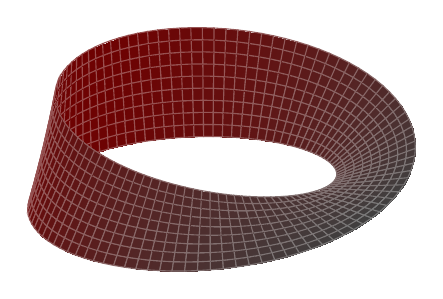
\begin{tikzpicture}[outer sep=1in,inner sep=1in]
    \begin{axis}[
        hide axis,
        view={40}{40},
        zmin=-0.5,
        zmax=0.5
    ]
      \addplot3 [
          surf,
          shader=faceted interp,
          faceted color={mapped color!70!white},
          point meta=x,
          samples=100,
          samples y=10,
          z buffer=sort,
          domain=0:360,
          y domain=-0.5:0.5
      ](
        {(1 + 0.5 * y * cos(0.5 * x))) * cos(x)},
        {(1 + 0.5 * y * cos(0.5 * x))) * sin(x)},
        {0.5 * y * sin(0.5 * x)}
      );
    \end{axis}
  \end{tikzpicture}
  & \\

  & &
\end{tabular}

\end{document}
